\chapter{Determinization in TAG Using Battleship}
\label{BattleshipInTAG}

\begin{abstract}
This chapter presents the TAG-based benchmark developed to study determinization quality in imperfect-information environments. Battleship is used as the reference case study because it provides a simple but representative hidden-position problem in which agents must reason about unknown spatial configurations using only partial observations.

The objective is not merely to implement Battleship in TAG, but to investigate how different determinization strategies influence the behavior and performance of simulation-based agents under uncertainty. Three strategies are introduced and compared: a naive random baseline, a constraint-based approach consistent with accumulated observations, and a heatmap-guided extension that biases simulations toward statistically plausible ship placements.

The full implementation is available on \hyperlink{https://github.com/jejeAKAgg/TFE26-093}{GitHub}\footnote{\url{https://github.com/jejeAKAgg/TFE26-093}}, which includes the \LaTeX{} source for this thesis alongside the TAG and Ludii implementations as Git submodules.
\end{abstract}


%%% 3.1 %%%
\section{Battleship as an Imperfect-Information Benchmark}
\label{sec:battleship_benchmark}

Battleship is a two-player hidden-information game played on separate grids. Before the game begins, each player secretly places a fleet of ships of varying sizes on their own board. During gameplay, players alternately target cells on the opponent's grid and receive binary feedback indicating whether the shot was a hit or a miss. The objective is to locate and destroy all opponent ships before losing one's own fleet.

Several characteristics make Battleship particularly suitable as a benchmark for imperfect-information reasoning. First, the game contains no stochastic events after initialization: uncertainty originates entirely from hidden information rather than randomness. This means that any performance difference between determinization strategies can be attributed directly to hidden-state reconstruction quality rather than to interactions with external randomness. Second, the hidden information concerns unknown spatial positions rather than hidden identities, making the game representative of the hidden Where category introduced in Chapter~\ref{Background}. Third, observations accumulate progressively throughout gameplay, continuously reducing the set of plausible opponent configurations and providing an increasingly informative constraint set for the determinization engine.

From an AI perspective, Battleship therefore naturally defines a constraint satisfaction problem over partially observed states. Every observed hit or miss restricts the set of valid ship placements consistent with the information available to the player. Simulation-based agents must consequently reason not only about future actions, but also about coherent hypotheses regarding the hidden configuration of the opponent's board. This is precisely the setting in which the quality of determinization is most consequential: an agent that generates incoherent hypotheses will simulate futures that could never correspond to the true game state, while an agent that generates well-constrained hypotheses will concentrate its search effort on plausible worlds.

Battleship was also selected for practical methodological reasons. Its rules are simple enough to allow controlled implementations in both TAG and Ludii while still capturing the core hidden-information challenges studied in this thesis, making the game well suited for isolating the effects of determinization mechanisms independently from more complex gameplay systems.

\begin{figure}[H]
    \centering % Centre l'ensemble des deux images sur la largeur de la page
    
    % Première image (gauche)
    \begin{minipage}[H]{0.45\textwidth}
        \centering
        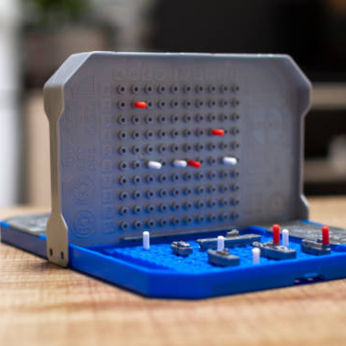
\includegraphics[width=0.7\textwidth]{figs/background/battleshipREAL.png}
    \end{minipage}
    \hfill % Crée l'espace entre les deux images
    % Deuxième image (droite)
    \begin{minipage}[H]{0.45\textwidth}
        \centering
        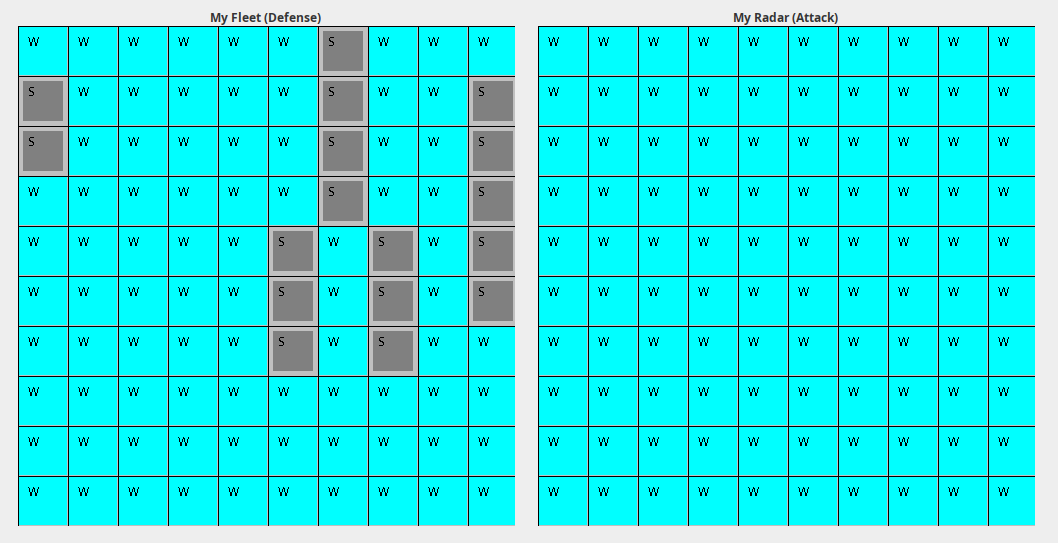
\includegraphics[width=1\textwidth]{figs/background/battleshipTAG.png}
    \end{minipage}

    \vspace{0.15cm} % Petit espace vertical avant la légende
    \captionsetup{justification=centering}
    \caption{Left: the physical Battleship board game. Right: the TAG graphical interface for the Battleship implementation developed in this thesis. The shot-tracking grid (right) records the acting player's observations; the ship grid (left) contains the true hidden fleet, masked from the opponent during play.}
    \label{fig:real_battleship_and_TAG_battleship}
\end{figure}

%%% 3.2 %%%
\section{Battleship Implementation in TAG}
\label{sec:battleship_tag_impl}

The Battleship benchmark was implemented in TAG using the standard three-component architecture described in Chapter~\ref{Background}. A game state class stores all information required to represent the current situation: separate ship grids and shot-tracking grids are maintained for each player. The ship grids contain the true hidden fleet configurations and are never exposed directly to the opposing agent; the shot-tracking grids store only the information revealed through previous actions, namely confirmed hits and misses. Remaining ship health values are maintained as auxiliary counters to allow the end-condition check to run in constant time rather than requiring a full grid scan at every move.

Game progression is handled by a forward model that generates all legal firing actions corresponding to untargeted cells on the opponent's grid. When an action is executed, both the hidden ship grid and the visible shot-tracking grid are updated according to the shot outcome. Hits and misses are therefore recorded incrementally as play progresses, continuously constraining the set of plausible opponent configurations available to the acting player. A separate parameter object stores the configurable properties of the game, including board dimensions and fleet composition, and is shared between the forward model and the determinization engine to ensure that all generated hypotheses remain consistent with the official game configuration.

The critical architectural contribution of this implementation lies not in the game logic itself but in how game-state copies are generated during simulations. In standard perfect-information environments, agents can safely reason over exact copies of the game state. In Battleship, directly copying the hidden opponent grid would expose privileged information during search. The state-copying mechanism therefore generates hypothetical hidden configurations consistent with the observations available to the requesting player, rather than simply duplicating the true state. The design of this mechanism is described in detail in the following section.


%%% 3.3 %%%
\section{Constraint-Based Determinization}
\label{sec:constraint_det}

The core contribution of the TAG benchmark lies in the determinization mechanism used during simulation-time state copying. Rather than exposing the true hidden opponent grid to search agents, the system generates hypothetical ship configurations that remain consistent with the observations available to the acting player.

The determinization process operates on two sources of information accumulated during gameplay. A \textit{hitMap} records every cell where the presence of an opponent ship has been confirmed through a successful shot. A \textit{missMap} records every cell where a shot has returned a negative result, confirming the absence of a ship. Together, these structures define a set of spatial constraints describing precisely which hidden configurations remain compatible with the player's accumulated observations. Figure~\ref{fig:det_pipeline} illustrates the overall pipeline from game observation to hypothesis generation.

\begin{figure}[H]
    \centering
    % TODO: Insert determinization pipeline diagram.
    % Suggested layout: left box "Player observations (hits + misses)" ->
    % arrow to center box "Constraint-Based Engine (CSP solver)" ->
    % arrow to right box "Coherent hypothesis (hypothetical grid)" ->
    % arrow down to "Injected into simulation copy"
    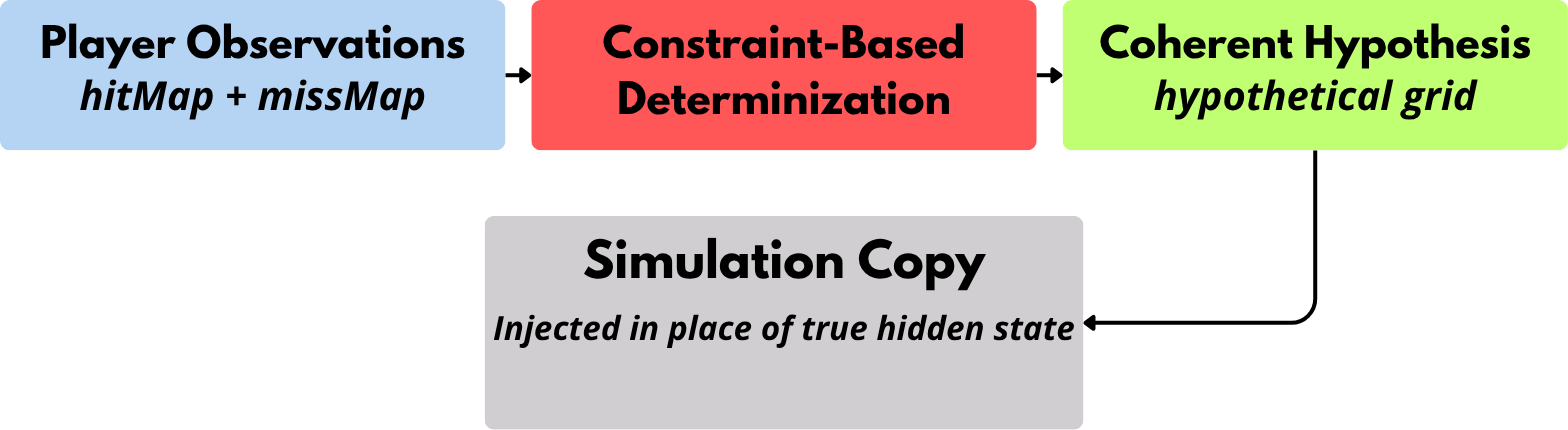
\includegraphics[width=1.00\textwidth]{figs/background/det_pipeline.png}
    \captionsetup{justification=centering}
    \caption{The constraint-based determinization pipeline. Accumulated hits and misses are used as spatial constraints to guide hypothesis generation. The engine produces a coherent hypothetical opponent grid that is injected into the simulation copy instead of the true hidden state.}
    \label{fig:det_pipeline}
\end{figure}

When a simulation copy is requested, the determinization engine constructs a hypothetical opponent grid satisfying these constraints. Ship placements conflicting with previously observed misses are rejected, while observed hits must remain covered by at least one valid ship placement. The generated hypothesis therefore represents a plausible hidden state consistent with the information available to the player at the time of the simulation.

The generation process can be interpreted as a constrained placement problem in which ships are placed sequentially. A placement is valid only if it remains within the board boundaries, does not overlap with any previously placed ship, and remains compatible with all entries in both the hitMap and the missMap. When multiple valid placements satisfy the current constraints, the engine samples among them in order to preserve diversity across simulations, preventing agents from repeatedly reasoning over a single deterministic hypothetical world. Figure~\ref{fig:det_example} illustrates an example of a coherent hypothetical configuration generated from partial observations.

\begin{figure}[H]
    \centering
    % TODO: Insert example of constraint-based determinization.
    % Suggested layout: 10x10 grid showing hit cells (red), miss cells (grey X),
    % and hypothesized ship placement (blue) consistent with all observations.
    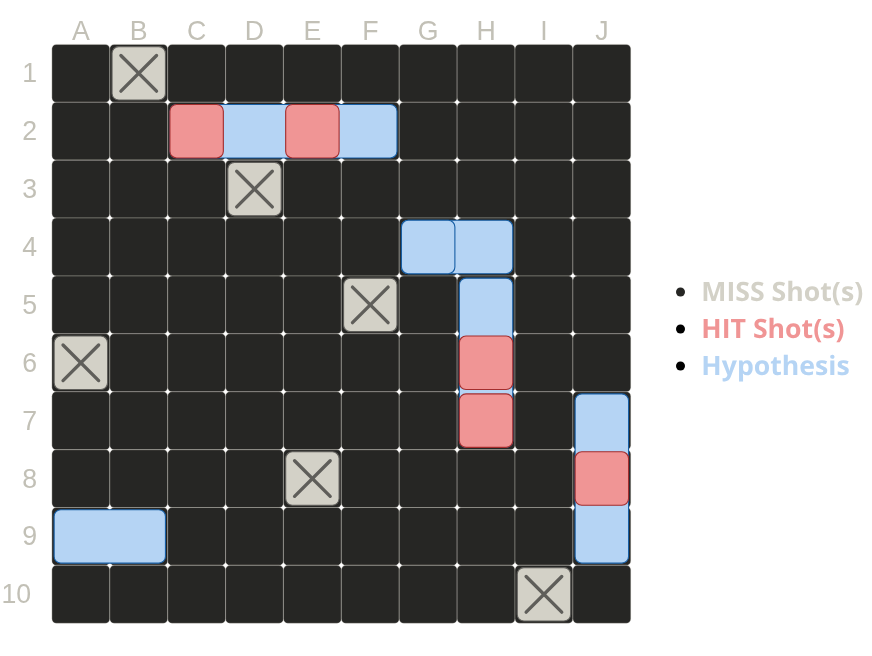
\includegraphics[width=0.65\textwidth]{figs/background/det_example.png}
    \captionsetup{justification=centering}
    \caption{Example of a constraint-based hypothetical configuration. Red cells are confirmed hits; grey cells are confirmed misses. The hypothesized fleet placement (blue) covers all hit cells and avoids all miss cells, representing one plausible world consistent with the agent's observations.}
    \label{fig:det_example}
\end{figure}

Unlike exact belief-state methods~\cite{morenville2024beliefsg,morenville2025belief_constraints}, the proposed approach does not attempt to enumerate or maintain the full distribution of possible hidden configurations. Instead, it approximates uncertainty through repeated generation of coherent hypothetical states during simulation. This makes the method computationally tractable while still preserving consistency with observed information. From a search perspective, the determinization engine acts as an intermediate layer between the true hidden game state and the simulation-based agent: the quality of the generated hypothetical states directly influences the quality of the forward simulations performed during search.


%%% 3.4 %%%
\section{Determinization Strategies}
\label{sec:det_strategies}

In order to evaluate the impact of hidden-state reconstruction quality on imperfect-information search, three determinization strategies were implemented in the TAG Battleship benchmark. Each strategy defines how hypothetical opponent ship configurations are generated during simulation-time state copying. The three approaches progressively increase the amount of information exploited from previous observations, making it possible to isolate the effect of increasingly informed determinization mechanisms while keeping the underlying search algorithms unchanged.

\subsection{Random Determinization}
\label{sec:random_det}

Random Determinization serves as the lower-bound baseline strategy. Hypothetical opponent ship configurations are generated through unconstrained random placement that respects only the structural rules of Battleship: board boundaries, ship sizes, orientations, and the non-overlap constraint. Hits and misses recorded during gameplay are entirely ignored when constructing the hypothetical opponent grid, so generated states may contradict information already revealed to the player, for instance by placing ships on cells previously observed as misses or by leaving known hit cells uncovered. This strategy therefore provides the worst-case reference for evaluating whether more informed determinizations improve simulation quality and, in turn, decision quality.

\subsection{Constraint-Based Determinization}
\label{sec:csp_det}

Constraint-Based Determinization incorporates the full set of observations accumulated during gameplay. The generated hidden configuration must remain consistent with all known hits and misses recorded in the player's shot-tracking grid. Cells marked as misses define forbidden positions; cells marked as hits must be covered by at least one ship in the generated hypothesis; all ships must additionally satisfy the standard placement constraints of remaining within the board, respecting their predefined lengths, and avoiding overlap with other ships.

Whenever several placements satisfy the current constraints, the engine samples among valid possibilities in order to preserve diversity across simulations. This allows agents to reason over multiple coherent hypothetical worlds rather than repeatedly reasoning from the same reconstructed configuration. The expected benefit of this strategy is improved simulation reliability: since the generated states no longer contradict previous observations, search algorithms evaluate actions in worlds that could plausibly correspond to the true hidden board, providing a genuine strategic signal rather than noise.

\subsection{Heatmap-Guided Determinization}
\label{sec:heatmap_det}

Heatmap-Guided Determinization extends the constraint-based strategy by estimating a probabilistic spatial prior over the opponent's grid. Rather than relying on a single coherent hypothesis per simulation copy, the engine first runs the constraint-based generator a large number of times to build a heatmap. Each sampled configuration contributes to this heatmap by incrementing a counter for every cell it occupies; the final heatmap is obtained by normalizing these counts over all samples. Cells with higher values correspond to locations that are more frequently occupied across the sampled configurations and therefore more likely to contain a ship according to the constraint-based prior.

This heatmap is then used to guide both determinization and action selection toward statistically plausible regions of the board. Rather than treating all constraint-consistent placements equally, the strategy weights sampling toward configurations that concentrate ships in high-probability zones, combining logical consistency with a lightweight approximation of the underlying belief distribution.

\begin{figure}[H]
    \centering
    % TODO: Insert heatmap visualization.
    % Suggested: 10x10 grid with a colour gradient from white (low probability)
    % to dark red (high probability), showing how probability concentrates
    % near known hit cells and around coherent ship-length continuations.
    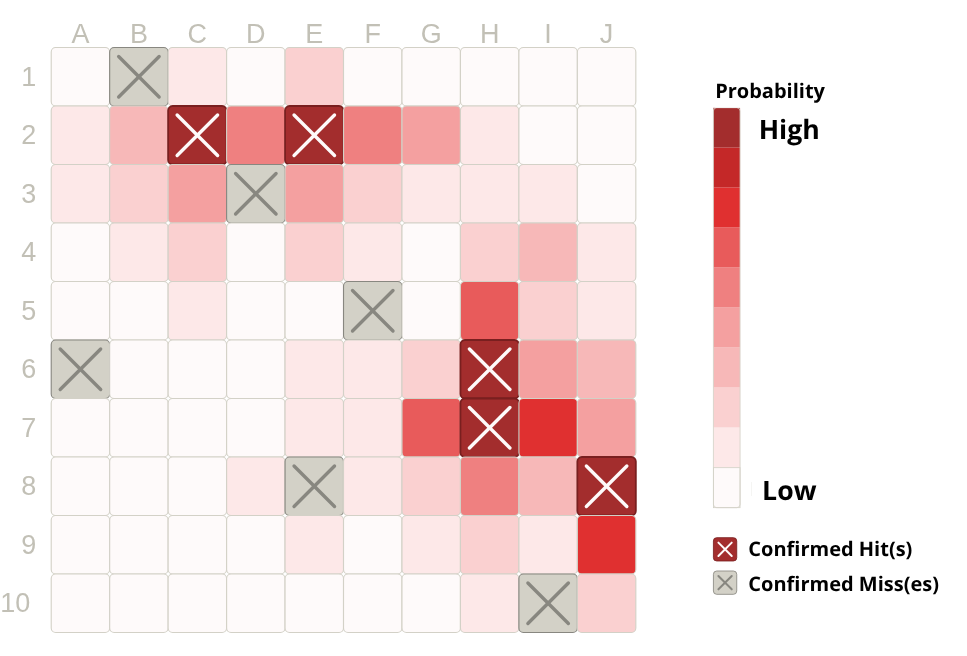
\includegraphics[width=0.7\textwidth]{figs/background/heatmap_example.png}
    \captionsetup{justification=centering}
    \caption{Example probabilistic heatmap produced by the Heatmap-Guided strategy after a partial game. Warmer colours indicate cells more frequently occupied across sampled constraint-consistent configurations. Probability concentrates near confirmed hit cells and along their plausible continuations.}
    \label{fig:heatmap_example}
\end{figure}



The central tradeoff of this strategy is computational cost. Building the heatmap requires running the constraint-based solver a large number of times before each decision, substantially increasing the time required to produce a simulation-ready copy of the game state. Agents that rely heavily on generating many simulations within a fixed time budget may therefore afford fewer iterations per move under this strategy, potentially offsetting the benefit of higher-quality individual simulations. The experiments in Section~\ref{sec:results} quantify this tradeoff directly.


%%% 3.5 %%%
\section{Experimental Setup}
\label{sec:exp_setup}

This section describes the experimental protocol used to evaluate the impact of determinization quality on simulation-based agents in the TAG Battleship benchmark. The experiments were designed to compare the three strategies introduced in Section~\ref{sec:det_strategies} while keeping the underlying search algorithms and game environment unchanged.

\subsection{Tournament Protocol}

The evaluation follows a round-robin tournament format in which every pair of agents competes in both player positions. For each matchup, agents alternate between playing first and second in order to control for first-player bias effects. Battleship is particularly sensitive to turn order because the first player always obtains the first opportunity to fire, accumulating hit and miss information one step ahead of the opponent. Each matchup consists of 100 games per direction, for a total of 200 games per pair, and the experiments are repeated independently for each of the three determinization strategies. This protocol makes it possible to isolate the impact of the determinization mechanism itself while preserving identical gameplay conditions across all comparisons.

\subsection{Evaluated Agents}

The benchmark evaluates five simulation-based agents representative of common General Game Playing approaches. The \textbf{Random} agent selects legal actions uniformly at random and never queries the game state, making it the primary control for validating that performance differences are genuinely attributable to determinization quality. \textbf{OSLA} applies a one-step lookahead heuristic, evaluating each legal action through a single forward simulation and selecting the highest-scoring immediate outcome. \textbf{RMHC} maintains a rolling horizon of candidate action sequences and optimizes them through repeated random mutation, relying on many forward simulations per decision step. \textbf{IS-MCTS} builds a search tree across multiple determinizations by sampling a new hypothetical world at each simulation step, aggregating results to identify the best action. \textbf{MAST} extends IS-MCTS by maintaining move-average statistics across rollouts to bias action selection toward historically effective moves.

Each agent is evaluated under all three determinization strategies, and search-based agents are additionally run under three thinking-time budgets of 100\,ms, 500\,ms, 1000\,ms and 5000\,ms per move. This multi-budget design allows the interaction between computational resources and determinization quality to be studied, in particular whether additional simulation time amplifies or compensates for the differences between strategies.

\subsection{Evaluation Metrics}

The experiments measure both gameplay performance and computational behavior in order to characterize the full impact of each determinization strategy.

The primary gameplay metric is win rate: the fraction of games won by an agent across all its matchups under a given strategy. As a secondary gameplay metric, the remaining ship health difference at the end of each game is recorded to assess how dominant or competitive individual matches are, providing a finer-grained view of agent strength than win rate alone.

On the computational side, three metrics are tracked for each strategy. Copy latency measures the average time in nanoseconds required to produce a single simulation-ready game-state copy, capturing the overhead introduced by the constraint solver relative to a raw copy. Search effort counts the average number of ship-placement attempts required by the engine before a valid constraint-consistent configuration is found, reflecting the difficulty of the constraint satisfaction problem as a function of game progression. Finally, the determinization success rate records the proportion of copy calls that result in a fully coherent hypothesis rather than a fallback to unconstrained random placement, validating the robustness of the constraint-based and heatmap-guided implementations as the game advances and the constraint set grows.

Together, these metrics make it possible to study not only whether informed determinizations improve agent performance, but also the computational tradeoffs they introduce.

\newpage

%%% 3.6 %%%
\section{Experimental Results}
\label{sec:results}

This section presents the experimental results obtained on the TAG 
Battleship benchmark. All experiments were conducted on the Dragon2 
computing cluster at UCLouvain. The cluster consists of 17 computing 
nodes, each equipped with two Intel Skylake Xeon 6142 processors 
(16 cores, 2.6 GHz); 15 nodes have 192 GB of RAM and 2 nodes have 
384 GB, all with 3.3 TB of local scratch space. Two additional nodes 
equipped with two Intel Skylake Xeon 6126 processors (12 cores, 
2.6 GHz) each host two NVIDIA Tesla V100 GPUs (5120 CUDA cores, 
16 GB HBM2, 7.5 TFlops double precision).%
\footnote{Full hardware specifications are available at the CÉCI 
documentation: \url{https://www.ceci-hpc.be/clusters/dragon2/}}

\subsection{Overall Agent Performance}
\label{subsec:overall}

The first set of experiments evaluates the overall win rates achieved 
by each agent under the three determinization strategies. 
Table~\ref{tab:winrates} summarizes the results across all agent and 
strategy combinations.

\begin{table}[H]
\centering
\begin{tabular}{lccc}
\hline
\textbf{Agent} & \textbf{Random Det.} & \textbf{Constraint-Based Det.} 
               & \textbf{Heatmap-Guided Det.} \\
\hline
Random  & $\approx 44\%$ & $\approx 2\%$  & $\approx 2\%$  \\
OSLA    & $\approx 53\%$ & $\approx 87\%$ & $\approx 87\%$ \\
RMHC    & $\approx 53\%$ & $\approx 87\%$ & $\approx 87\%$ \\
IS-MCTS & $\approx 49\%$ & $\approx 37\%$ & $\approx 37\%$ \\
MAST    & $\approx 50\%$ & $\approx 38\%$ & $\approx 37\%$ \\
\hline
\end{tabular}
\captionsetup{justification=centering}
\caption{Average win rates by agent and determinization strategy 
         (1000\,ms budget, rounded).}
\label{tab:winrates}
\end{table}

The results reveal a striking and consistent pattern. Under Random 
Determinization, all five agents perform near chance level, with win 
rates ranging from 44\% to 53\%. While small deviations from 50\% are 
visible, notably OSLA and RMHC at 53\% and Random at 44\%, no 
agent demonstrates meaningful strategic advantage at this stage. 
IS-MCTS, which builds a search tree through repeated simulations, 
achieves the same result as the Random agent, which picks actions 
blindly. This uniformity is not surprising: it is exactly the outcome 
that Random Determinization was designed to demonstrate. Because each 
simulation is performed in a world where ships are placed with no 
regard for observed hits and misses, the resulting action evaluations 
carry no information about the true hidden configuration. Aggregating 
many such simulations, as IS-MCTS does, only produces a more confident 
wrong answer. The principle is simple: garbage in, garbage out.

The transition to Constraint-Based Determinization produces an 
immediate and dramatic reversal. OSLA and RMHC emerge as the strongest 
agents, achieving win rates of approximately 87\%. The Random agent, 
as expected, shows no improvement: since it never consults the game 
state to make decisions, the quality of the copy it receives is 
entirely irrelevant to its behavior. This invariance of the Random 
agent across all three strategies serves as a critical sanity check, 
confirming that the observed performance differences in other agents 
are genuinely caused by the determinization mechanism rather than by 
any confounding factor in the experimental setup.

\begin{figure}[H]
    \centering
    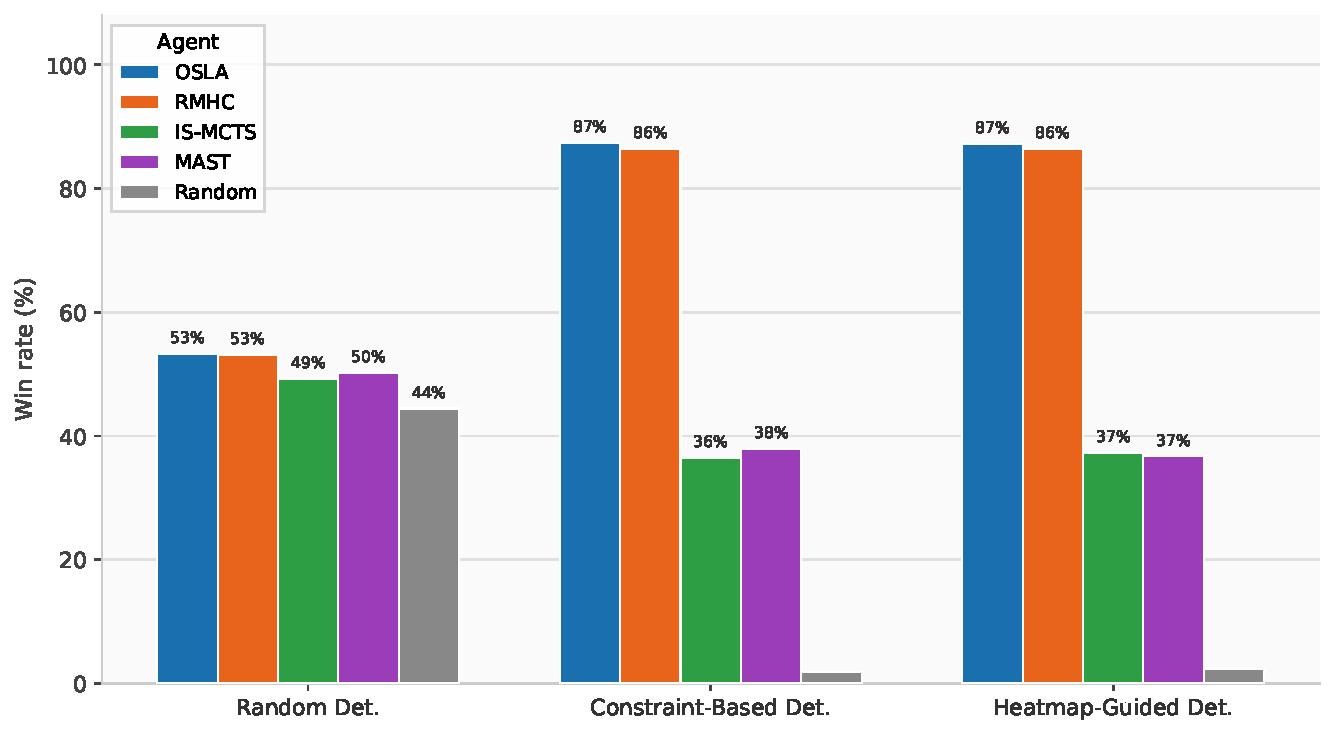
\includegraphics[width=1\textwidth]{Sections/4_TAG/figs/winrate_barplot.pdf}
    \captionsetup{justification=centering}
    \caption{Average win rates per agent under the three determinization 
    strategies (1000\,ms budget).}
    \label{fig:winrate_barplot}
\end{figure}

The strong performance of OSLA under Constraint-Based Determinization 
is particularly noteworthy, given that it only looks one step ahead. 
When that single forward step is simulated in a world that is logically 
consistent with the observed game history, the heuristic evaluation 
becomes meaningful: the agent can reliably distinguish between targeting 
a cell near a confirmed hit and targeting a region already identified as 
empty. This is precisely the spatial reasoning that constraint-based 
filtering enables, and it allows even a shallow agent to make 
well-informed decisions. The results suggest that in imperfect-information 
environments with structured spatial uncertainty, simulation consistency 
matters more than search depth. IS-MCTS and MAST, by contrast, achieve win rates of approximately 37\% under Constraint-Based Determinization which is lower than under Random Determinization. This apparent paradox is explained by the tournament 
structure: OSLA and RMHC now dominate every matchup so decisively that 
IS-MCTS and MAST lose the majority of their games against them. 

\newpage

\begin{figure}[H]
    \centering
    
    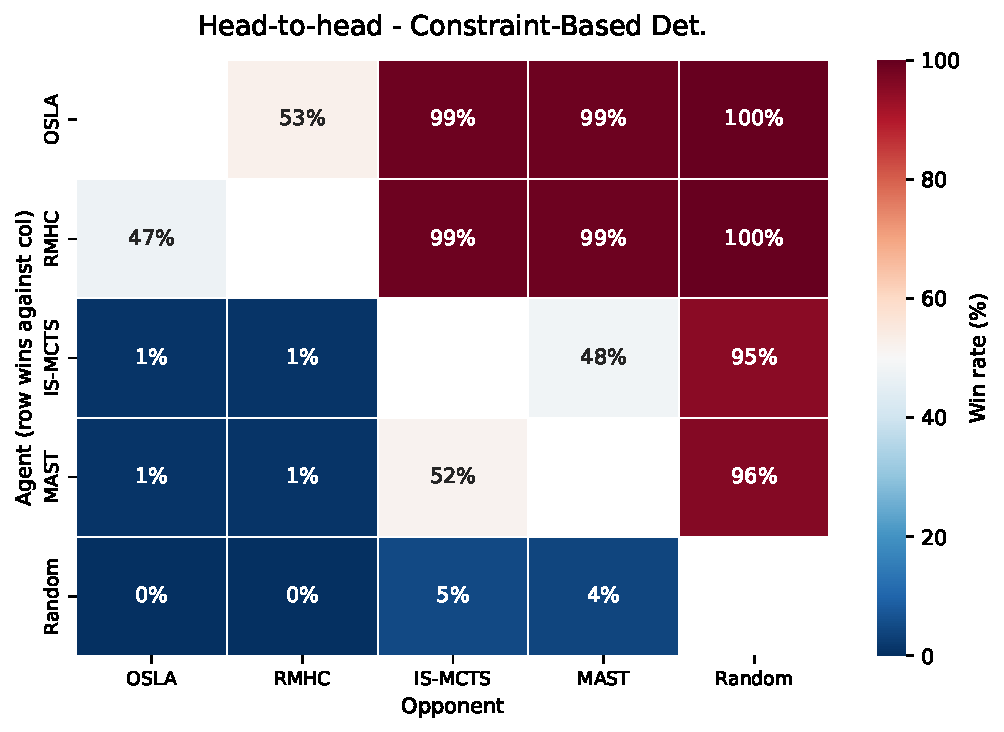
\includegraphics[width=\textwidth]{Sections/4_TAG/figs/heatmap_constraintbased_det.pdf}
    
    \vspace{0.3cm}
    
    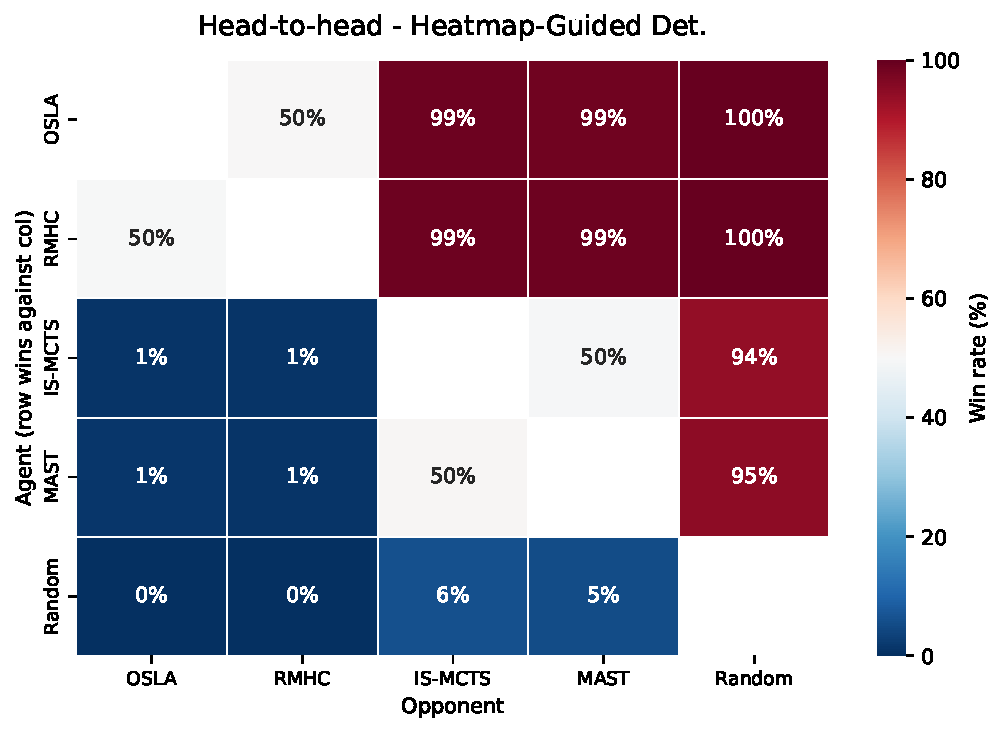
\includegraphics[width=\textwidth]{Sections/4_TAG/figs/heatmap_heatmapguided_det.pdf}
    
    \vspace{0.15cm}
    \captionsetup{justification=centering}
    \caption{Head-to-head win rates under Constraint-Based (top) and 
    Heatmap-Guided (bottom) Determinization (1000\,ms budget). 
    OSLA and RMHC dominate every matchup against IS-MCTS and MAST 
    under both strategies, and the pairwise patterns are 
    indistinguishable, confirming that the heatmap provides no 
    measurable advantage in head-to-head outcomes at this time budget.}
    \label{fig:heatmap_both}
\end{figure}

In direct matchups, OSLA wins over 98\% of its games against IS-MCTS. The 
constraint-based hypotheses benefit OSLA and RMHC directly at each 
evaluation step, whereas IS-MCTS still performs its rollouts using 
uniform random target selection. A deeper search tree built over coherent 
worlds provides limited benefit when the terminal evaluations are guided 
by random play.

Under Heatmap-Guided Determinization, no agent shows a meaningful 
change relative to Constraint-Based Determinization. OSLA and RMHC 
maintain their win rates near 87\%, while IS-MCTS and MAST remain near 
37\% regardless of the number of heatmap sampling iterations used 
(10, 50, or 100). The heatmap therefore provides no measurable 
performance benefit in this experimental setting. One possible explanation 
is that the heatmap improves the spatial prior used during 
determinization, but does not address the fundamental limitation of 
IS-MCTS and MAST: their rollout policies remain uniform random, so the 
quality of individual simulations is not improved by a more informed 
prior over ship positions.

The head-to-head matrices confirm this pattern at the pairwise 
level: under Constraint-Based and Heatmap-Guided Determinization, 
OSLA and RMHC win over 99\% of their games against IS-MCTS and 
MAST, while Random loses virtually all matchups against the 
stronger agents.

\newpage

\subsection{Impact of Computational Budget}
\label{subsec:budget}

The second set of experiments studies how performance evolves as the 
thinking-time budget increases from 100\,ms to 500\,ms, 1000\,ms, and 
5000\,ms, under both Constraint-Based and Heatmap-Guided Determinization.

\begin{figure}[H]
    \centering
    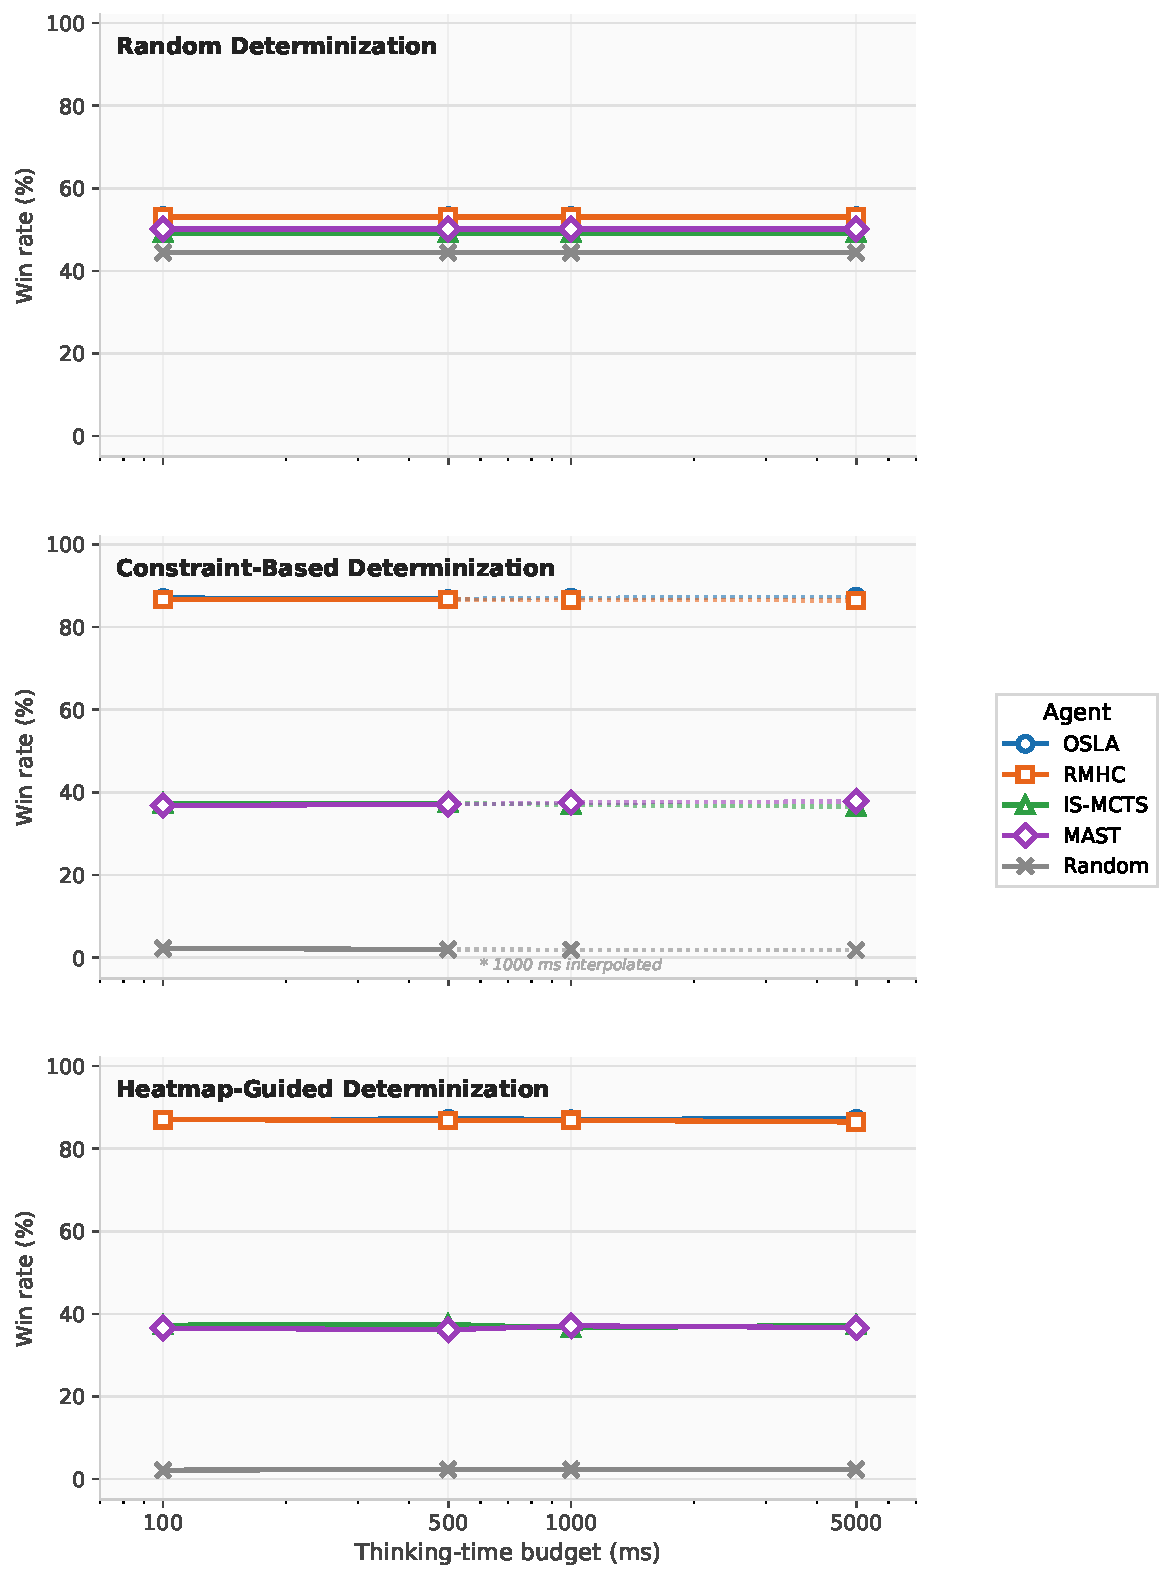
\includegraphics[width=0.9\textwidth]{Sections/4_TAG/figs/winrate_vs_time.pdf}
    \captionsetup{justification=centering}
    \caption{Win rate as a function of thinking-time budget for each 
    agent under the three determinization strategies. Color identifies 
    the agent; line style identifies the strategy. Under all strategies, 
    no agent shows a meaningful performance change as the budget 
    increases from 100\,ms to 5000\,ms.}
    \label{fig:winrate_vs_time}
\end{figure}

The results are unambiguous: the budget has no measurable effect on 
agent performance under any strategy. OSLA and RMHC maintain win rates 
of approximately 87\% across all four time budgets, and IS-MCTS and 
MAST remain near 37\% regardless of how much additional computation 
time they receive.

This invariance is itself an informative result. For OSLA, the absence 
of a budget effect is expected: since it evaluates only a single forward 
step per action, additional time beyond the minimum required to assess 
all legal moves provides no benefit. For IS-MCTS and MAST, the result 
is more significant: more simulation time does not compensate for the 
structural limitation of random rollouts. Building a deeper search tree 
over constraint-consistent worlds still produces unreliable value 
estimates if the terminal evaluations are guided by uniform random play. 
This confirms that the bottleneck for these agents is not computational 
budget but rollout quality.

\subsection{Game Outcome Analysis}
\label{subsec:outcomes}

Beyond win rates, the experiments also characterise the nature and 
margin of game outcomes across the three determinization strategies.

\begin{figure}[H]
    \centering
    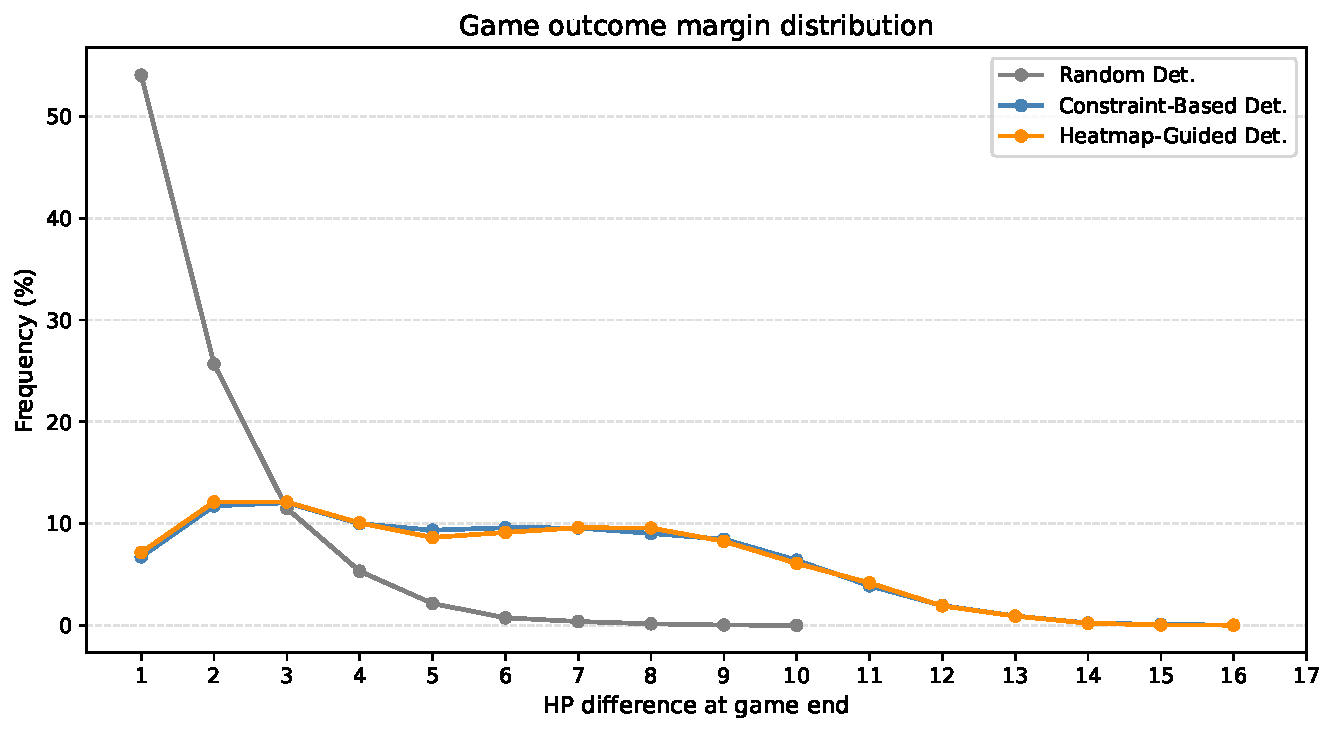
\includegraphics[width=\textwidth]{Sections/4_TAG/figs/drama_distribution.pdf}
    \captionsetup{justification=centering}
    \caption{Distribution of the HP difference between winner and loser 
    at the end of each game, shown for all three determinization strategies. 
    Under Random Determinization, the majority of games end with a margin 
    of 1 HP; under Constraint-Based and Heatmap-Guided Determinization, 
    the distribution flattens toward larger margins (1000ms budget).}
    \label{fig:drama}
\end{figure}

Figure~\ref{fig:drama} characterises the nature of game outcomes across 
strategies. Under Random Determinization, the majority of games end with 
a margin of just 1\,HP, indicating closely contested matches in which 
neither agent holds a consistent advantage. Under Constraint-Based and 
Heatmap-Guided Determinization, the distribution flattens and shifts 
toward larger margins, with many games ending with differences of 
5\,HP or more.

The winner's remaining HP distribution tells the same story from the 
other side: winners under Constraint-Based and Heatmap-Guided 
Determinization finish with substantially more HP than under Random 
Determinization, reflecting the fact that informed agents do not merely 
win more often, they win more decisively. This result is consistent 
with the head-to-head analysis: when OSLA or RMHC faces IS-MCTS or the 
Random agent under an informed strategy, the outcome is rarely close. 
The combination of coherent simulation hypotheses and direct spatial 
exploitation at each evaluation step produces a systematic and 
one-sided advantage.

\begin{figure}[H]
    \centering
    
    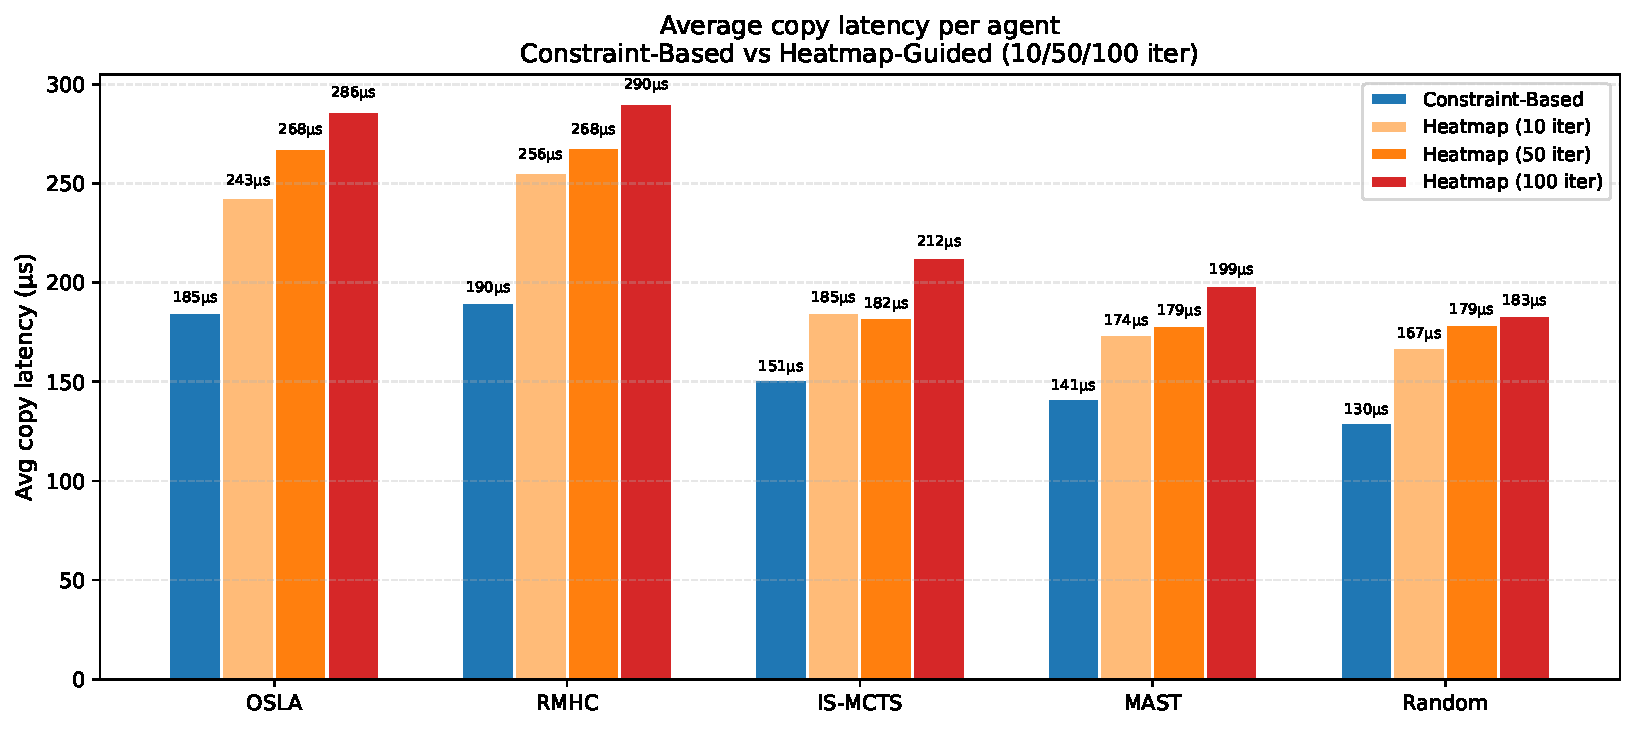
\includegraphics[width=\textwidth]{Sections/4_TAG/figs/copy_latency.pdf}
    
    \vspace{0.3cm}
    
    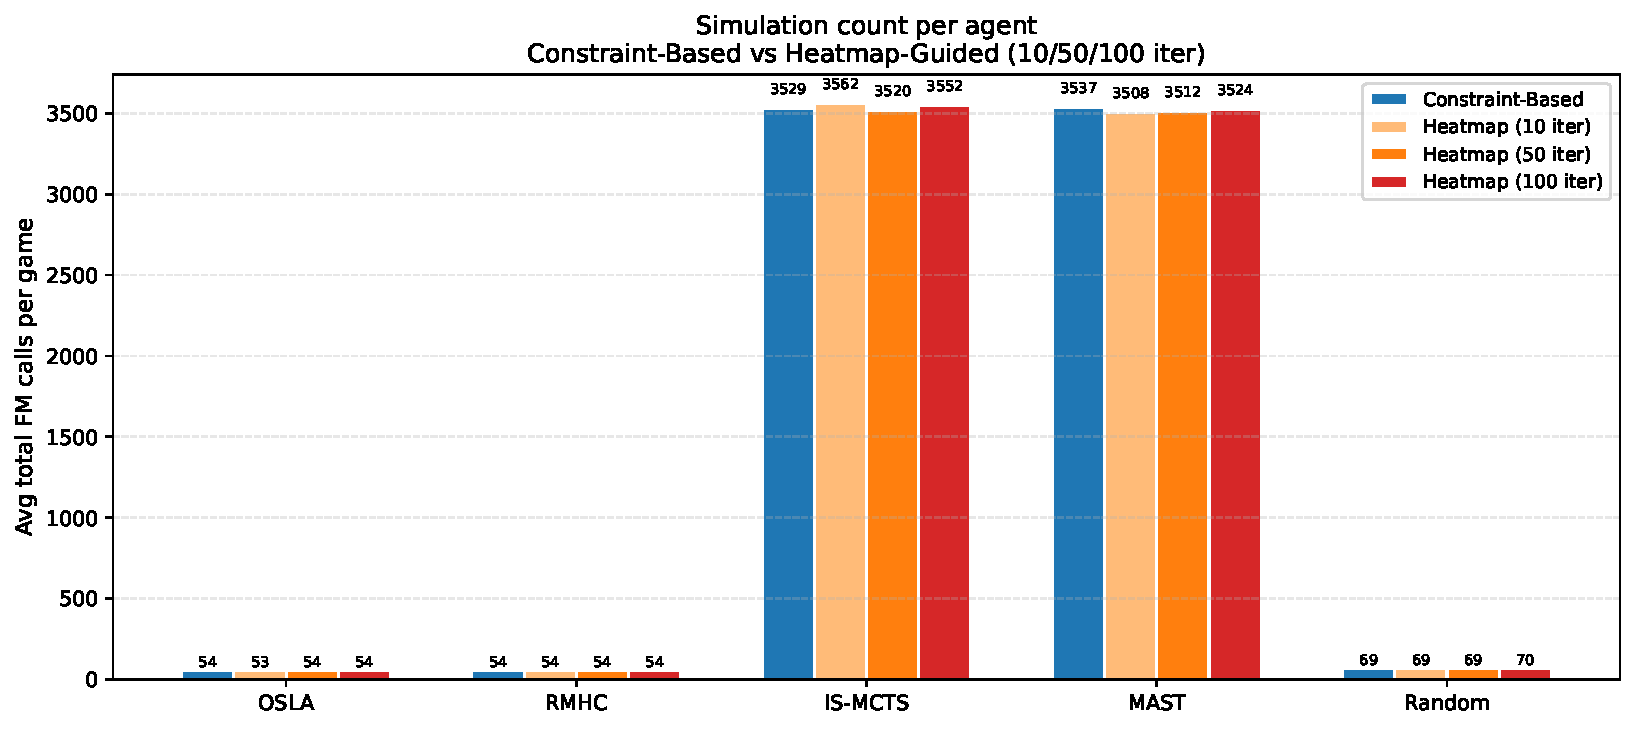
\includegraphics[width=\textwidth]{Sections/4_TAG/figs/fm_calls.pdf}
    
    \vspace{0.15cm}
    \captionsetup{justification=centering}
    \caption{Average copy latency (top) and total forward model calls per game 
    (bottom) for Constraint-Based and Heatmap-Guided Determinization 
    (10, 50, and 100 heatmap iterations). Despite a higher copy latency under Heatmap-Guided Determinization, the number of forward model calls remains comparable across all strategies.}
    \label{fig:copy_latency_and_fm_calls}
\end{figure}

Figure~\ref{fig:copy_latency_and_fm_calls} 
confirms that the budget invariance is not due to insufficient 
simulation depth. Despite Heatmap-Guided Determinization 
introducing a copy latency approximately 55\% higher than 
Constraint-Based, the total number of forward model calls per 
game remains comparable across both strategies, indicating that 
the 1000\,ms budget absorbs the overhead without reducing 
simulation count.


%%% 3.7 %%%
\section{Discussion}
\label{sec:tag_discussion}

The experiments conducted on the TAG Battleship benchmark highlight the central importance of determinization quality in imperfect-information simulation-based search. The results suggest that simulation consistency plays a more decisive role than search algorithm sophistication in hidden-information environments. Random Determinization frequently generates hypothetical states that contradict previously observed information, forcing search algorithms to reason over implausible worlds and producing no useful strategic signal regardless of how many simulations are run. Constraint-Based Determinization restricts simulations to configurations compatible with known hits and misses, producing search trajectories that accurately reflect the uncertainty actually faced by the player and enabling even shallow agents such as OSLA to perform strongly. The Heatmap-Guided strategy further refines this process by weighting simulations toward statistically plausible regions of the board, providing an additional benefit for tree-search agents at the cost of increased per-copy computational overhead.

The experiments also reveal an important observation about the relationship between determinization quality and the search algorithm. One might expect that a more powerful algorithm such as IS-MCTS, which samples many worlds and aggregates their results, would be more robust to poor determinizations than a shallow agent like OSLA. The results show the opposite: under Random Determinization, IS-MCTS performs no better than the Random agent, while OSLA achieves strong performance as soon as the determinizations become constraint-consistent. Aggregating many incoherent simulations does not produce a useful signal; it merely produces a more confident wrong answer. The gains from more sophisticated search are therefore contingent on the quality of the hypothetical worlds those algorithms reason about.

Another observation concerns the independence between the determinization mechanism and the search algorithm. The same agent exhibits substantially different behavior depending on the quality of the hypothetical states it receives during simulation. This reinforces one of the central claims of this thesis: in imperfect-information environments, hidden-state reconstruction is a fundamental component of the simulation architecture rather than a secondary implementation detail. Improving determinization quality is a more reliable path to better agent performance than increasing search depth, at least in the hidden-position setting studied here.

More broadly, the TAG implementation demonstrates that preserving uncertainty during simulation-time state copying can significantly improve imperfect-information reasoning while remaining compatible with general simulation-based search techniques. The benchmark therefore provides a useful reference architecture for studying hidden-information handling in General Game Playing systems. These observations directly motivate the next part of this thesis: while TAG enables explicit control over player-specific state copying through its code-first architecture, Ludii currently relies on more generic context-copy mechanisms. The following chapters investigate how determinization techniques inspired by this benchmark can be integrated into Ludii in order to preserve hidden-information uncertainty during simulation-based search.